% 英文で執筆する場合はクラスファイルへのオプションを[T,E]としてください.
% If you want to write your paper in English, pass to [T,E] options to document class.
\documentclass[T,J]{fose} % 「コンピュータソフトウェア」用のクラスファイルは compsoft です.
\taikai{2023} % 固定です.出版委員長が毎年変更してAuthor Kitを配布してください.

\usepackage [dvipdfmx] {graphicx}
\usepackage{multirow}
\usepackage{caption}

% ユーザが定義したマクロなどはここに置く.ただし学会誌のスタイルの
% 再定義は原則として避けること.

% 以下は説明のために使用したパッケージであるため,削除可能.
\usepackage{fancyvrb}
\usepackage{xurl}
\usepackage{cite}
\usepackage{color}
\usepackage{graphicx}
\usepackage{ascmac}
\usepackage{textcomp}
% \usepackage[dvipdfmx]{color} クラッシュしていてなくても動くのでコメントアウト


\newcommand{\todo}[1]{\colorbox{yellow}{{\bf TODO}:}{\color{red} {\textbf{[#1]}}}}
\newcommand{\done}[2]{\colorbox{green}{{\bf DONE}:} {\textbf{[#1]}}}
\newcommand{\checked}[3]{\colorbox{red}{ここまでチェック済み}}

\begin{document}

% 論文のタイトル
\title{Scratchにおけるプログラム類似度とオブジェクト\\動作軌跡類似度の乖離の分析}
% 以下の \etitle(と\@etitle)はFOSE論文フォーマット独自のマクロです.
% FOSEに投稿した論文を発展させてコンピュータソフトウェアに投稿される場合はコメントアウトしてください.
% \setetitleは奇数ページのヘッダに表示する文字列(\etitle)を設定するためのマクロです.
% タイトルが2行に渡る場合は "\\" を 使用することで任意の位置で改行をすることができます.
\setetitle{An Analysis of Program Similarity and Object Motion Trajectory Similarity between Scratch Works}
%\setetitle{Long Long Long Long Long Long \\ Long Long Long Long Long \\ Long Long Long Long Long Long Long Long Long Long Long Long Paper Title}

% タイトル,著者などが複数行にわたり,論文冒頭の著者名が日本語アブストと重複して描画された場合に以下のコメントアウトを外してください.
%\longtitle

% 著者
% 和文論文の場合,姓と名の間には半角スペースを入れ,
% 複数の著者の間は全角スペースで区切る
%
\author{岡本 圭悟 伊原 彰紀
%
% ここにタイトル英訳 (英文の場合は和訳) を書く.
% 英語タイトルは論文1ページ目左下,著者らの名前・所属一覧の一番上に表示される
%
\ejtitle{\etitle}
% 上記\setetitle中で改行した場合は "\etitle" を削除し,改行(\\)を入れていないタイトルを記載してください.
% \ejtitleは1ページ目左下に挿入されるタイトルとして使用されます.
% また,"\etitle"はFOSE論文フォーマット独自のマクロです.
%\ejtitle{\etitle}
%
% ここに著者英文表記 および
% 所属 (和文および英文) を書く.
% 複数著者の所属はまとめてよい.
%
% 複数著者の所属は以下のようにまとめてよい.
\shozoku{Keigo Okamoto, Akinori Ihara}{和歌山大学システム工学部}
{Faculty of Systems Engineering, Wakayama University}
}

%
% 和文アブストラクト
% In English paper, content of Jabstract will be ignored. 
\Jabstract{
Scratchでは,プログラムの類似性とオブジェクト動作軌跡の類似性が乖離する作品が存在し,その乖離が多様な実装方法を有する作品収集に有効であることもあるが,検索において期待しない作品が収集されることもある.
本研究では,ケーススタディとして4,000件のScratch作品を対象に類似性の乖離する作品を分析した結果,プログラムが類似してオブジェクト動作軌跡が類似しない作品は全体の約1\%,オブジェクト動作軌跡が類似してプログラムが類似しない作品は全体の約28\%存在することを確認し,多様な実装方法を有する作品収集に有効であることが多いことを明らかにした.
}
%
% 英文アブストラクト(本サンプルの原論文にはなし)
%\Eabstract{
%\todo{英文アブスト}
%}
%

\maketitle \thispagestyle {empty}
%%%%%%%%%%%%%%%%%%%%%%
\vspace{-7pt}
\section{はじめに}
%%%%%%%%%%%%%%%%%%%%%%
%杉浦学,松澤芳昭,岡田健,大岩元.アルゴリズム構築能力育成の導入教育:実作業による概念理解に基づくアルゴリズム構築体験とその効果.情報処理学会論文誌,Vol.49,No.10,pp.3409-3427,2008.
%森秀樹, 杉澤学, 張海, 前迫孝憲.Scratchを用いた小学校プログラミング授業の実践 : 小学生を対象としたプログラミング教育の再考(教育実践研究論文).日本教育工学論文誌,Vol.34, No.4, pp.387\UTF{2013}394, 2011.

ビジュアルプログラミング言語Scratchにおいて,ユーザは制作したプログラム作品をオンライン上に公開できる.Scratchは自然言語による作品検索サービスを提供しており,ユーザは公開済み作品の中から実現したい作品を検索し,実装の参考にしている\cite{Resnick_2009}.
%Mitchel Resnick, John Maloney, Andr´es Monroy-Hern´andez, Natalie Rusk, Evelyn Eastmond, Karen Brennan, Amon Millner, Eric Rosenbaum, Jay Saul Silver, Brian S Silverman, Yasmin Bettina Kafai, Scratch: Programming for all, Communications of the ACM, Vol.52, No.11, pp.60-67, 2009.
Scratch上で使用できるブロックは限られるため,検索によって類似するプログラムを含む作品やオブジェクトの描く動作軌跡が類似する作品が多数出力される.検索結果の中にはプログラムが類似していてもオブジェクトの動作軌跡が異なる作品もあり,同じ実装方法でも視覚的には異なる出力結果であるため,ユーザにとって学習の妨げになることが示唆される.一方,プログラムが異なってもオブジェクトの動作軌跡が類似する作品もあり,異なる実装方法で視覚的に同じ出力結果を再現できているため,ユーザにとって学習の参考になることが示唆される.先行研究\cite{Fukuchi2021}\cite{Mikura2022}ではこれらのプログラムの類似性とオブジェクト動作軌跡の類似性の乖離が存在することは確認されているが,その程度は明らかとなっていない.

本研究では,Scratchにおけるプログラムの類似性とオブジェクト動作軌跡の類似性の乖離の程度を調べ,ユーザの学習の参考になる作品を増加させるために,Scratch上から条件に基づいて収集した4,000件の作品を対象に,プログラムが類似するか否か,オブジェクトの動作軌跡が類似するか否かの4種類に分類し,類似性が乖離する作品の特徴を分析する.

\vspace{-7pt}
%%%%%%%%%%%%%%%%%%%%%%
\section{動作軌跡類似度とプログラム類似度の分析}\label{sec:Analysis}
%%%%%%%%%%%%%%%%%%%%%%

%%%%%%%%%%%%%%%%%%%%%%
\subsection{動作軌跡類似度とプログラム類似度}\label{sec:Similarity}
%%%%%%%%%%%%%%%%%%%%%%

本研究は先行研究\cite{Fukuchi2021}\cite{Mikura2022}に基づき,動作軌跡の類似度を,DTW(Dynamic time warping)を用いて算出したDTW距離とし,プログラムの類似度を抽象構文木間の編集距離とする.

\vspace{-10pt}
\subsection{分析手法}
本分析では,ブロック数が5以上の作品を対象とする.ただし,動作軌跡の計算が複雑化するため,並列に動作するブロックおよび独自に定義されたブロックが存在する作品は除外する.条件をみたす作品を公開日時の古い順に4,000件収集した.

収集作品間の動作軌跡類似度,プログラム類似度を総当たりで測定し,先行研究で示された閾値に基づいて作品のプログラムが類似するか否か,オブジェクト動作軌跡が類似するか否かの4種類に分類する.

%,DTW距離の算出結果について分析を行った.定量分析では,距離を昇順に並べたある2点の傾きから距離が収束する値を求めることで,類似しない動作が抽出されるおおよその距離を明らかにした.定性分析では,定量分析で明らかにした距離以下の動作を提示し,動作の類似性を評価するアンケートを実施することで,類似動作を抽出可能な距離を4種類の入力それぞれについて明らかにした.本研究では,先行研究で示された4種類の入力と類似する動作を抽出可能な距離4つのうち,最もDTW距離の小さい2.2を動作軌跡が類似する境界値とする.
\vspace{-10pt}
\subsection{分析結果}\label{subsec:result}

%------------------------
\begin{figure}[t]
	\centering
	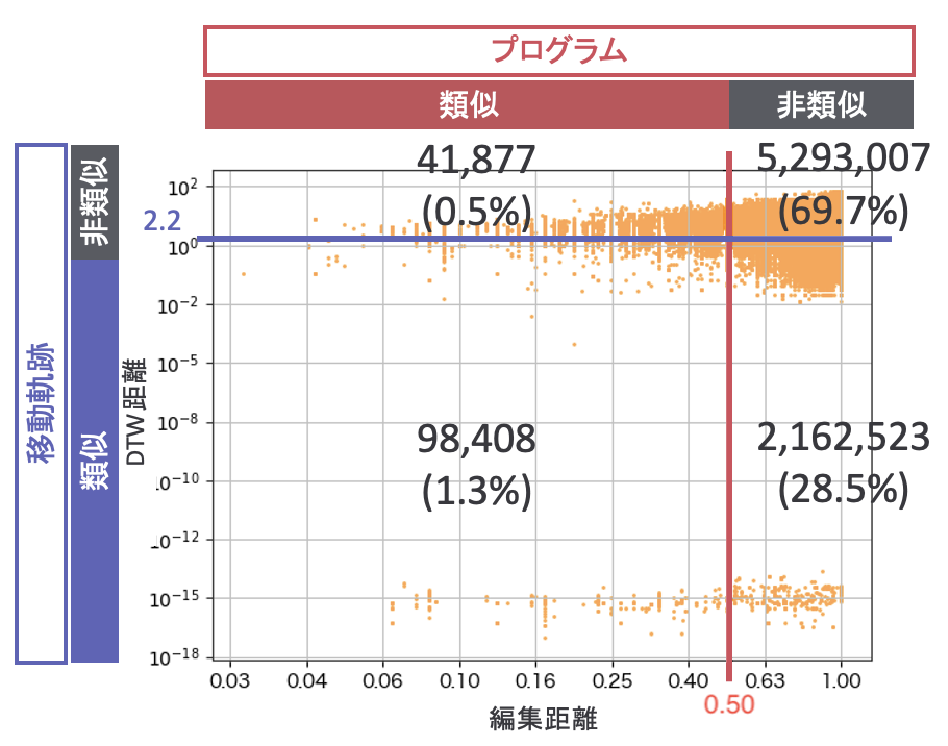
\includegraphics[width=1.0\linewidth]{Okamoto_fig/result.pdf}
	\caption{DTW距離と編集距離の関係性を示した散布図}
	\label{fig:out-nolimit}
\end{figure}
%------------------------

%-------------------------
%-------------------------

図\ref{fig:out-nolimit}は,分析対象とする4,000作品を総当たりに編集距離とDTW距離を計測した結果を散布図で示す.横軸は編集距離、縦軸はDTW距離を示す.それぞれの軸は対数表記している.散布図の1点は,2つの作品間の類似度を計測した作品対の結果を表す.また,編集距離とDTW距離の境界値を赤線で示す.この境界線に基づき,4,000作品の中から類似度を算出できた7,595,815作品対を4つに分類する.

図\ref{fig:out-nolimit}中の4つの各象限の数値は,各象限に分類された作品対の数と割合を示す.分析の結果,移動軌跡が類似する作品は全体の29.8\%(=1.3+28.5)も存在し,そのうちプログラムが類似しない作品対は28.5\%も存在していた.ビジュアルプログラミングは作品が単純であるため類似することが多いとはいえ,異なる実装方法で実現していることが多く,検索によって収集作品を参照することで,ユーザは多様な実装方法の学習が可能であることが示唆される.
%無作為に取得した作品中で,25\%以上の作品対が存在することからこれは意味のある数値と言え,Scratchでは動作軌跡の類似する作品が多様な実装方法で作成されていることが明らかとなった.
%また,動作軌跡が類似せず,プログラムが類似する作品対は約0.5\%であり,大きな課題ではないと考える.
%散布図中の第2象限は動作軌跡もプログラムも類似しない,第2象限は動作軌跡は類似しないが,プログラムは類似する,第3象限は動作軌跡もプログラムも類似する,第4象限は動作軌跡は類似するが,プログラムが類似しないことをそれぞれ意味する.

%図中の1点は1つの作品対であることを表す.また,\ref{subsec:approach}で示した境界値を図中の線で示しており,この境界線に基づいて作品を4種類に分類した.






% \todo{いらない気がする}表\ref{table:program-classification}は4つに分類された作品対のうち,それぞれの分類に含まれる作品の数を示している.本ケーススタディで分類した作品数は4000であるため,表\ref{table:programs-classification}より,分類された作品の数に大きな違いはないことがわかる.

% 表\ref{table:program-length}は4つに分類された作品のプログラムに含まれるブロック数(ブロック長)の平均値を示している.この結果より,4つに分類された作品群の間で,ブロック長には大きな違いがないことがわかる.

%-------------------
% \begin{table}[t]
%     \centering
%     \caption{分類別作品対の数の比較}
%     \begin{tabular}{c|l|r|r}
%         \hline
%         \multicolumn{2}{c|}{}& \multicolumn{2}{c}{プログラム} \\ \cline{3-4}
%         \multicolumn{2}{c|}{}& \multicolumn{1}{c|}{類似する} & \multicolumn{1}{c}{類似しない} \\
%         \hline
%         動作&類似しない & 41,877 & 5,293,007 \\
%         軌跡&類似する & 98,408 & 2,162,523 \\ \cline{2-4}
%         \hline
%     \end{tabular}
% %    \captionsetup{skip=5pt}
%     \label{table:programs-classification}

% \vspace{2mm}

%     \centering
%     \caption{分類別作品数の比較}
%     \begin{tabular}{c|l|r|r}
%         \hline
%         \multicolumn{2}{c|}{}& \multicolumn{2}{c}{プログラム} \\ \cline{3-4}
%         \multicolumn{2}{c|}{}& \multicolumn{1}{c|}{類似する} & \multicolumn{1}{c}{類似しない} \\
%         \hline
%         動作&類似しない & 3,017 & 3,889 \\
%         軌跡&類似する & 2,842 & 3,603 \\
%         \hline
%     \end{tabular}
%     \captionsetup{skip=5pt}
%     \label{table:program-classification}

% \vspace{2mm}

%     \centering
%     \caption{分類別ブロック長平均値の比較}
%     \begin{tabular}{c|l|r|r}
%         \hline
%         \multicolumn{2}{c|}{}& \multicolumn{2}{c}{プログラム} \\ \cline{3-4}
%         \multicolumn{2}{c|}{}& \multicolumn{1}{c|}{類似する} & \multicolumn{1}{c}{類似しない} \\
%         \hline
%         動作&類似しない & 15.4 & 18.0 \\
%         軌跡&類似する & 15.5 & 16.7 \\
%         \hline
%     \end{tabular}
%     \captionsetup{skip=5pt}
%     \label{table:program-length}
% \end{table}
%-------------------


% 第3象限と第4象限の作品対は共にDTW距離が小さいが,編集距離が大きい第4象限に比べて,第3象限の方がDTW距離が小さいため,作品として類似している.\todo{効果量次第?効果量が小さい場合は,DTWが小さくてもプログラムが違うので多様性のある実装が多い,みたいなことを言う.}

% 編集距離の分布には確実な差異が存在することが示されたが,その差異は実質的には小さいことが示唆される.

% 第象限と第3象限の作品対は共に編集距離が小さいが,DTW距離が大きい第2象限に比べて,第3象限の方が編集距離が小さいため,作品として類似している.

% \todo{効果量次第?効果量が小さい場合は,プログラムが似通っていてもDTWは違うので,検索が難しい,みたいなことを言う?}

%-------------------------
%-------------------------
\vspace{-10pt}
\subsection{考察}
% 本節では,\ref{subsec:result}の結果を踏まえて,編集距離によるプログラムの類似性の妥当性について考察する.
% 動作軌跡とプログラムのそれぞれについて考察を述べる.
% \subsubsection{動作軌跡の類似性}
% \ref{subsec:result}の結果より,動作軌跡が類似しない作品対が全体の半数以上存在することが判明した.このことから,作品全体で動作軌跡を比較しても動作軌跡が類似しない作品が多くあることがわかる.そのため,動作軌跡を部分的に切り取って類似性を測定することで,動作軌跡が類似する作品対が増加することが示唆される.
% \subsubsection{プログラムの類似性}
\ref{subsec:result}節の結果より,動作軌跡が類似していても,プログラムが類似しない作品対が多く存在するため,その要因について事例を挙げて考察する.
図\ref{fig:pattern2-1}に,動作軌跡が類似してもプログラムが類似しなかった事例を示す.この作品対のプログラムは,それぞれ制御文を利用しているためプログラム構造は類似しているが,(2)のプログラムでは座標移動に関わるブロック以外のブロックも多数使用しているため,プログラムが類似していない.

% 結果として,動作・制御ブロック以外の抽象化を行った時に最も分類の精度が良くなったが,動作ブロックと制御ブロックを基準にしており,一般化に向けて適切とは言えないため,最終的にその次に精度が高かった意味が類似するブロックの抽象化を最適な抽象化手法とした.

座標移動に関わるブロック以外のブロックを抽象化(削除)しても動作軌跡に影響はないため,本研究では抽象化することでプログラムの類似性が向上すると示唆する.ただし,抽象化によって実装の多様性が失われることが考えられるため,プログラムの類似性を向上しつつ,実装の多様性を失わない抽象化手法を今後の研究で検討する.

\begin{figure}[t]
	\centering
	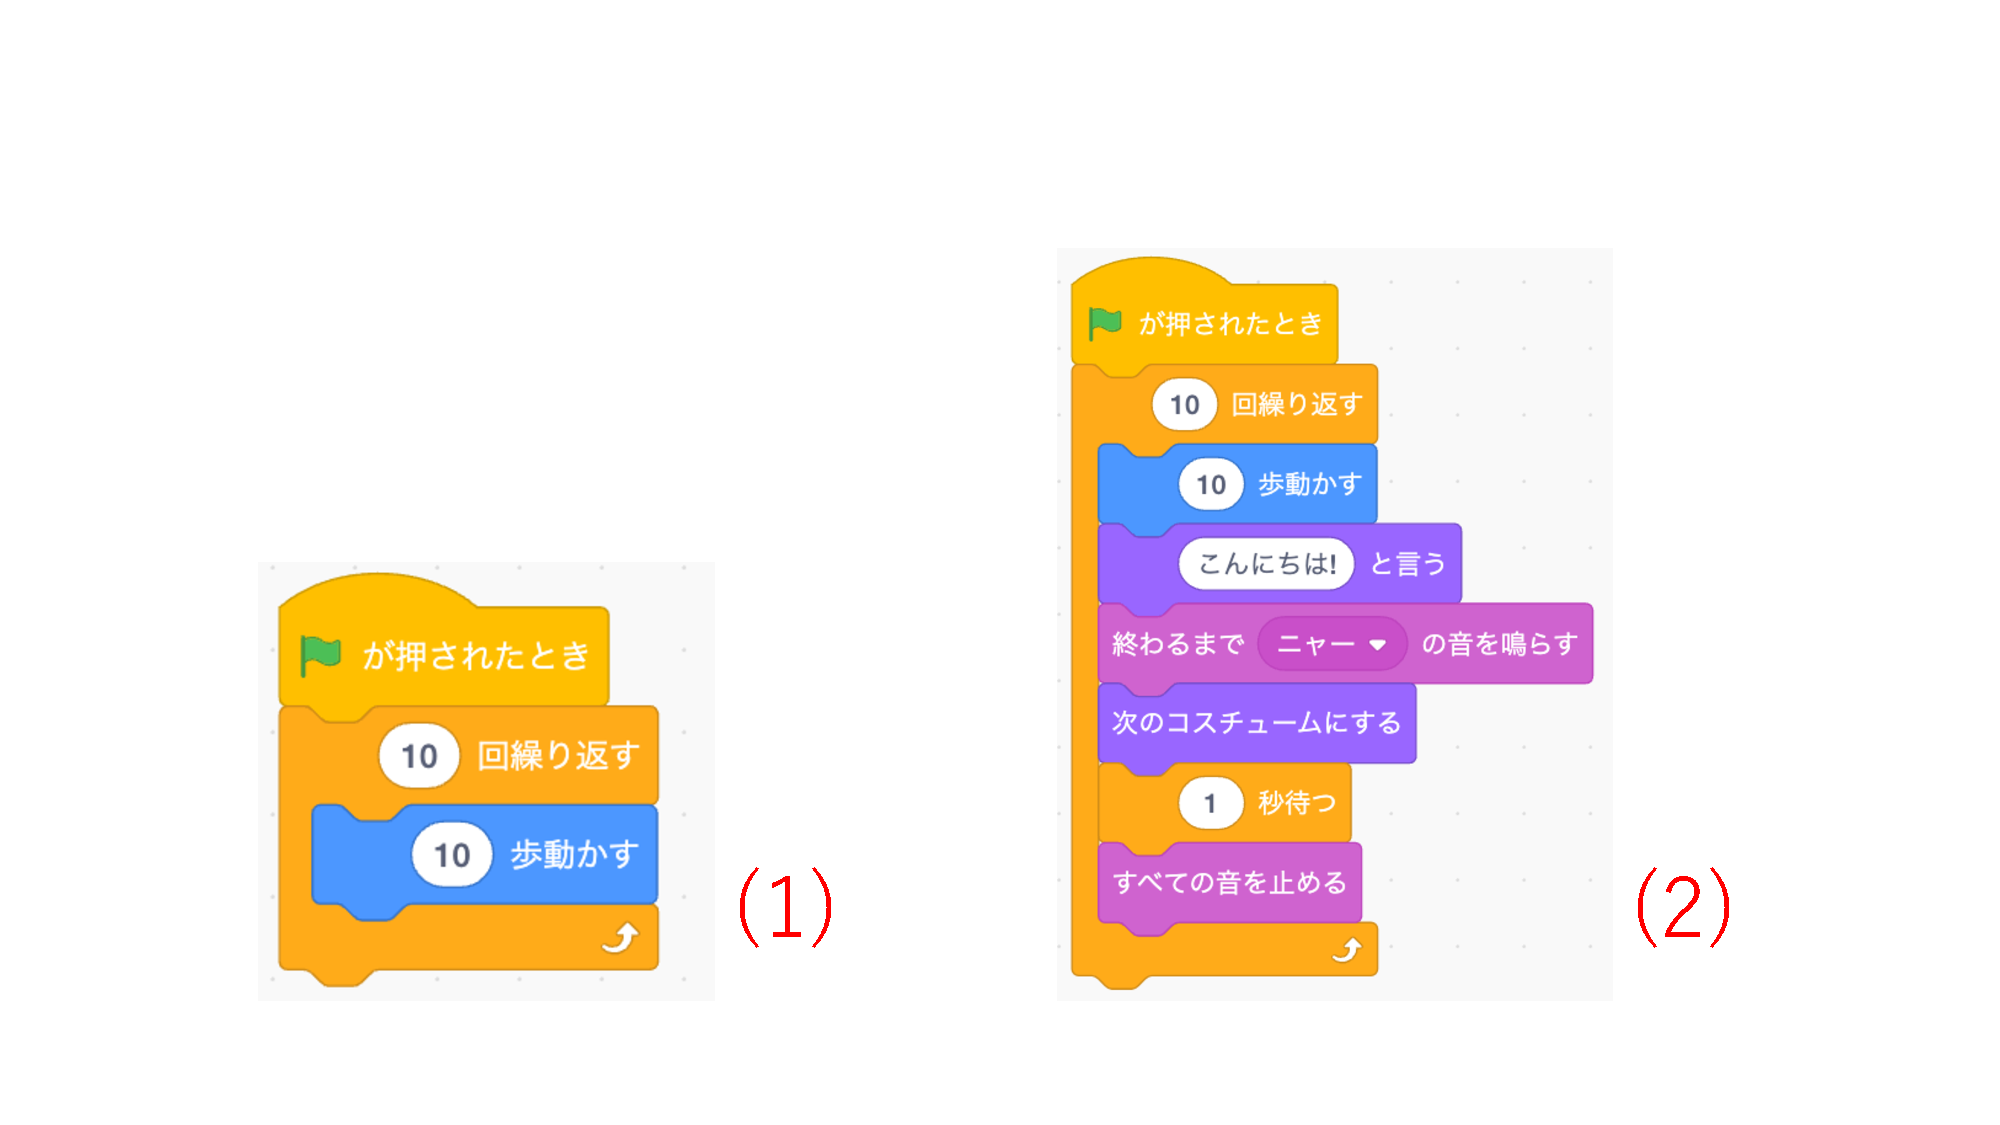
\includegraphics[width=1.0\linewidth]{Okamoto_fig/pattern2-1.pdf}
	\caption{オブジェクト動作軌跡は類似するが,プログラムが類似していない作品の事例}
   \vspace{-2mm}
	\label{fig:pattern2-1}
\end{figure}



\vspace{-7pt}
%%%%%%%%%%%%%%%%%%%%%%%
\section{おわりに}\label{sec:con}
%%%%%%%%%%%%%%%%%%%%%%%

本研究では,4,000件のScratch作品を類似性に基づいて4種類に分類した.結果,動作軌跡が類似し,プログラムが多様な作品が多いことを明らかにし,その特徴も事例から明らかにした.今後は類似する動作軌跡を持つ作品の中でユーザのレベルに応じたプログラムの実装パターンを特定する.

% \textbf{謝辞}\
% ありがとうございます
% \todo{謝辞}


%\begin{adjustvboxheight} % needed only when Appendix follows
\bibliographystyle{junsrt}
\bibliography{okamoto}

%\end{adjustvboxheight} % needed only when Appendix follows

% 以下はbibtexを使用しない場合の例です.
% 332行目と333行目をコメントアウトしてから使用してください.
% なお,この例では年数順に文献が並んでいるので適切な並び順ではありません.
%\begin{adjustvboxheight} % needed only when Appendix follows
%\begin{thebibliography}{9}
%\bibitem{fose2021} 名倉 正剛,関澤 俊弦 編:ソフトウェア工学の基礎28,日本ソフトウェア科学会{\em FOSE2021}, 近代科学社, 2021.
%\bibitem{fose2022} 角田 雅照,まつ本 真佑 編:ソフトウェア工学の基礎29,日本ソフトウェア科学会{\em FOSE2022}, 近代科学社, 2022.
%\bibitem{fose2023} 吉田 則裕,槇原 絵里奈 編:ソフトウェア工学の基礎30,日本ソフトウェア科学会{\em FOSE2023}, 近代科学社, 2023. (to appear)
%\end{thebibliography}
%\end{adjustvboxheight} % needed only when Appendix follows

%以下は付録の例です.必要ならコメントアウトして使用してください.
%なお,その際には参考文献の前後にある adjustvboxheight 環境のコメントアウトを解除してください.
%\appendix
%\section{付録A} 
%これは付録の例です.

\end{document}


